% IEEE conference-format distillation of docs/PROJECT_PAPER.tex (the 47-page report).
% Every number here is the same number as in the report and the committed JSONs
% (docs/survey_validation.json, survey_extras.json, ablation_results.json,
% asr_fairness.json, backend/models/model_metadata.json). Build: latexmk -pdf IEEE_PAPER.tex
\documentclass[conference]{IEEEtran}
\IEEEoverridecommandlockouts
\usepackage[T1]{fontenc}
\usepackage[utf8]{inputenc}
\usepackage{cite}
\usepackage{amsmath,amssymb}
\usepackage{graphicx}
\usepackage{booktabs}
\usepackage{array}
\usepackage{url}
\usepackage{xcolor}
\usepackage[hidelinks]{hyperref}
\usepackage{microtype}
\graphicspath{{figures/}}
\def\BibTeX{{\rm B\kern-.05em{\sc i\kern-.025em b}\kern-.08em T\kern-.1667em\lower.7ex\hbox{E}\kern-.125emX}}

\begin{document}

\title{Measuring \emph{How} Children Play, Not Just How Long:\\
A Multimodal, Privacy-Conscious Screening System for Gaming Addiction with External Construct Validation}

\author{
\IEEEauthorblockN{Kaustubh Agarwal, Khushee P Kiran, Kanak Goyal, Vidisha Murali}
\IEEEauthorblockA{Department of Computer Science and Engineering, PES University, Bengaluru, India\\
Guide: Prof.\ Shridevi Sawant \quad Team PW26\_SAS-03\\
\texttt{github.com/kaustubhagarwal21/gaming-addiction-detection-capstone}}
}

\maketitle

\begin{abstract}
Consumer parental-control tools report \emph{how long} a child played; they cannot
distinguish three hours of healthy play from three hours of compulsive play. We present
a deployed, three-tier screening system --- a passive-capture Android child app, a cloud
ML backend, and a parent app --- that fuses three channels: ten \emph{measured}
behavioural features (late-night ratio, rapid re-logins, binges, streaks), calibrated
chat toxicity across English, romanised Hindi and Devanagari, and on-device
speech-to-text plus acoustic emotion. All models are lightweight, calibrated and
SHAP-explainable; raw audio is never retained. Each channel is evaluated on real
held-out data with bootstrap confidence intervals and one-component ablations
(chat PR-AUC $0.825$ in-domain, $\geq$$0.95$ alert precision on every register;
voice $0.574$ speaker-independent, exposing a 9-point leakage inflation in random splits).
Critically, we then validate the served risk score \emph{externally}: in an anonymous
adult IGDS9-SF survey ($87$ usable, $86$ scoreable), the score correlates with the clinical instrument at
Spearman $\rho{=}0.352$ ($95\%$ CI $[0.158,0.521]$), beats the self-reported screen-time
baseline on a paired bootstrap ($\Delta\rho{=}{+}0.195$, CI excluding zero), and the
signal is carried by \emph{pattern} features (composite $\rho{=}0.358$) rather than
\emph{volume} ($0.202$, CI including zero) --- the design premise confirmed rather than
assumed. The same study returns two results against the system (an unsupported genre
multiplier; four of five parent-facing proxy names failing to track their namesake
items), which we report and act on. An accent-fairness audit on 6{,}656 Indian-English
clips finds zero false toxicity alerts in every accent group but a coverage gap
(WER $35\%$ Dravidian $\rightarrow$ $61\%$ Tibeto-Burman). Limits are stated plainly:
behavioural training labels remain synthetic, caseness metrics are uncomputable at the
observed severity base rate, and the cohort is adults, not the adolescent target.
\end{abstract}

\begin{IEEEkeywords}
gaming disorder, screening, multimodal fusion, calibration, construct validity,
IGDS9-SF, toxicity detection, code-mixed Hindi, fairness, mobile health
\end{IEEEkeywords}

% =====================================================================
\section{Introduction}
Internet Gaming Disorder (IGD) is recognised behaviourally by DSM-5 and
ICD-11~\cite{icd11}: impaired control, escalating priority of gaming, continuation
despite harm. Parents notice late and from the outside. The two families of existing
tools each miss the pattern: self-report questionnaires require the child's honest
cooperation --- and denial is itself a diagnostic criterion --- while screen-time
counters measure volume, which is a weak correlate of severity. Prior computational
work either models survey data~\cite{huang2024,strojny2024} or reviews family
factors~\cite{ergin2025}; passive smartphone sensing of behaviour and mental state has
precedent in student populations~\cite{studentlife2014}, but none of this work deploys a
passive, multi-signal screen to a guardian.

We built and deployed such a system and, distinctively, evaluated it the way a
screening instrument should be: real data where it exists, stated limits where it
does not, and an external validation against a clinical instrument that could --- and
partly did --- fail. Contributions:
\begin{enumerate}
\item A deployed three-tier platform (two native Android apps, cloud Flask backend)
  with a train/serve-aligned behavioural pipeline: ten measured features are the only
  model inputs; ten psychometric proxies derived from them serve as explanations,
  keeping SHAP~\cite{shap2017} attributions non-circular.
\item An availability-weighted ensemble that renormalises over the channels present,
  with isotonic calibration (behaviour ECE $0.062\!\rightarrow\!0.015$) and a
  precision-first alert threshold chosen as a product decision, not a metric.
\item An India-ready abuse channel: dual-script Hindi trained on HASOC~\cite{hasoc2019}
  with a clean-Hindi counterweight~\cite{wikihi} that drains a measured script-level
  toxicity prior; a native Devanagari keyboard so canvas games are not blind spots;
  and an accent-fairness audit on Svarah~\cite{svarah2023}.
\item External construct validation of the served score against IGDS9-SF~\cite{igds9sf}
  in $87$ respondents, with incremental validity over screen time, a
  pattern-versus-volume decomposition, and two negative results reported.
\item An evaluation protocol designed to be falsifiable: speaker-independent splits, one-component
  ablations with bootstrap CIs, three transformer baselines, and continuous-integration
  guards that fail the build if the paper's numbers diverge from the committed data.
\end{enumerate}

% =====================================================================
\section{System Architecture}
\textbf{Data-collection tier (Child app).} A foreground service detects game sessions
from the foreground package (curated allowlist $\rightarrow$ OS game category
$\rightarrow$ parent override), records ten objective session features, captures typed
chat through a custom keyboard (IME) --- which, unlike the accessibility API, reads
text in canvas/engine games such as Roblox --- and an accessibility fallback, and
records short microphone segments only while a tracked game is foreground, gated by
voice-activity detection. Speech-to-text runs on-device (Vosk~\cite{vosk}, Indian
English); transcripts and a short WAV go over HTTPS; the server deletes audio after
feature extraction. Consent is versioned and fails closed; anti-tamper covers
force-stop, uninstall (optional Device Admin), and capture-permission revocation, each
raising a guardian alert rather than a silent gap.

\textbf{Serving tier.} A Flask backend (Render; Neon Postgres in production, SQLite in
development, one code path tested on both) scores each channel, fuses them, produces
SHAP explanations, raises alerts to every guardian device, runs a weekly drift monitor
(PSI/KS) against production, and exposes symmetric \emph{export} and \emph{delete}
endpoints sharing one table inventory.

\textbf{Presentation tier (Parent app).} Risk band with plain-language ``why'',
14-day trend, alerts with accurate/false-alarm verdicts feeding a Beta-posterior
threshold tuner (capped $\pm0.05$ per run, human-applied), nudges to the child, and a
``what we can and cannot see'' screen naming the blind spots.

% =====================================================================
\section{Methodology}
\subsection{Behavioural features and labels}
The model consumes ten \emph{objective} features: five volume (daily/weekly hours,
sessions/day, session duration, days/week) and five pattern (late-night ratio, longest
streak, binges/week, break between sessions, rapid re-login ratio). Ten psychometric
proxies (``craving'', ``tolerance'', \dots) are deterministic functions of these ten,
derived through one shared function at train and serve time; they are shown to parents
and never fed to the model. No public dataset pairs per-session device telemetry with
IGD labels --- we audited candidates and rejected two Kaggle sets after inspection
(synthetic provenance; engagement labels) --- so labels are \emph{synthetic screening
priors}, with play-time distributions grounded in a real survey of $13{,}464$ gamers
and the severity base rate ($6.4\%$ scoring $\geq$$36$) taken from the open $11{,}191$-row
release of a seven-country IGDS9-SF study of League of Legends players~\cite{igdslatam2024}. We state throughout that the resulting accuracy
bounds separability of the synthetic distribution, not clinical validity; \S\ref{sec:survey}
is where the score meets real labels.

\subsection{Models}
\textbf{Behaviour}: Random Forest (200 trees, depth 6) on the ten features, chosen by a
tabular bake-off, then isotonic-calibrated on a held-out split. \textbf{Chat}: TF-IDF
(word 1--2 + char\_wb 3--5 grams) $\rightarrow$ logistic regression $\rightarrow$
isotonic, trained on five real corpora --- Jigsaw~\cite{jigsaw2018},
CONDA in-game chat~\cite{conda2021}, Davidson~\cite{davidson2017}, HASOC 2019
Hindi~\cite{hasoc2019} in Devanagari and a colloquial romanisation, and a clean-Hindi
Wikipedia counterweight~\cite{wikihi} --- and noisy-OR fused with a curated
Hinglish/Devanagari lexicon screened against Bohra et al.~\cite{bohra2018}.
\textbf{Voice}: 36 acoustic features $\rightarrow$ HistGradientBoosting trained on
four real speech corpora (RAVDESS~\cite{ravdess2018}, CREMA-D~\cite{cremad2014},
EMO-DB~\cite{emodb2005}, URDU~\cite{urdu2018}; $9{,}817$ clips, 154 speakers, three
languages) through the exact serving extractor; plus the STT$\rightarrow$chat path.

\subsection{Fusion and alerting}
Session risk is a weighted fusion (prior $0.4/0.3/0.3$) \emph{renormalised over the
channels present}, so a missing modality contributes nothing rather than a false
neutral. Session chat risk is the \emph{maximum} per-message calibrated score. Alerts
fire at $0.95$, deliberately above best-F1 ($0.85$): at the realistic $\sim$$3.5\%$
toxic base rate a $0.5$ threshold yields precision $0.235$ --- three false alarms per
real one --- and parents stop reading alerts. All thresholds are environment-tunable.

\subsection{Evaluation protocol}
Every model is evaluated on held-out data it never trained on with recorded seeds.
Voice uses \emph{speaker-independent} splits; chat's headline is \emph{in-domain}
(CONDA validation split, $21.5\%$ toxic). Ablations remove one component per row on a
fixed test set with bootstrap $95\%$ CIs (1{,}000 resamples); ``better'' is claimed
only when intervals separate. MCC and PR-AUC are reported alongside F1 because base
rates are extreme. Calibration is shown directly (top-label ECE, reliability
diagrams), not only via Brier.

% =====================================================================
\section{Results}
\subsection{Per-channel results}
\textbf{Behaviour.} Test accuracy $0.916$, macro-F1 $0.918$, 5-fold CV
$0.921\pm0.002$ ($23{,}000$ / $5{,}750$ rows); errors fall only in \emph{adjacent}
bands. Isotonic calibration lowers Brier $0.134\!\rightarrow\!0.128$ and top-label
ECE $0.062\!\rightarrow\!0.015$ (worst-bin gap $0.50\!\rightarrow\!0.05$;
Fig.~\ref{fig:rel}). Ablation (Table~\ref{tab:abl}): an hours-only model reaches
$0.702$ and commits two-band errors every richer set avoids; the five pattern features
alone recover $0.902$ versus $0.871$ for the five volume features.

\textbf{Chat.} In-domain PR-AUC $0.825$ $[0.807,0.841]$; at the alert threshold,
precision $0.956$, recall $0.428$, MCC $0.589$ (Fig.~\ref{fig:pr}). Off-the-shelf
toxic-BERT~\cite{detoxify2020} scores $0.709$ on the same split. On the HASOC held-out
Hindi set (933 rows) the deployed pipeline reaches precision $0.968$ / recall $0.425$
(Devanagari) and $0.958$ / $0.366$ (romanised) at the unchanged $0.95$ threshold ---
from near-zero coverage before adoption. Removing CONDA domain data collapses PR-AUC to
$0.511$; removing char\_wb n-grams costs $0.031$; removing keyword fusion costs recall
$0.491\!\rightarrow\!0.434$ at equal precision.

\textbf{Voice.} Speaker-independent accuracy $0.574$, macro-F1 $0.568$ (chance
$0.25$); random splits had reported $0.657$, a 9-point speaker-leakage inflation we
corrected. The channel is deliberately tied-lowest in the fusion prior (0.3, with chat) and an optional
witness in fusion; frozen wav2vec~2.0 embeddings reach $0.776$ on the identical
split, so a distilled on-device encoder is the identified next step rather than a
claim of this paper.

\begin{table}[t]
\centering\footnotesize
\caption{Selected ablations (held-out; bootstrap 95\% CIs). One component removed
per row from the deployed recipe.}
\label{tab:abl}
\begin{tabular}{@{}llc@{}}
\toprule
Channel & Configuration & Metric \\
\midrule
Chat (PR-AUC) & full recipe (deployed) & $0.825$ $[0.807,0.841]$ \\
 & $-$ keyword fusion & $0.814$ $[0.796,0.830]$ \\
 & $-$ char\_wb n-grams & $0.794$ $[0.777,0.811]$ \\
 & $-$ Davidson corpus & $0.794$ $[0.775,0.812]$ \\
 & $-$ CONDA domain data & $\mathbf{0.511}$ $[0.487,0.535]$ \\
\midrule
Behaviour (acc.) & objective-10 (deployed) & $0.916$ \\
 & all-20 incl.\ derived proxies & $0.919$ \\
 & pattern features only (5) & $0.902$ \\
 & volume features only (5) & $0.871$ \\
 & screen-time only (baseline) & $\mathbf{0.702}$ \\
\midrule
Voice (acc.) & full (36 feats, 4 corpora) & $0.562$ \\
 & $-$ augmentation & $0.566$ (neutral) \\
 & English-only corpora & $0.546$ \\
 & 17-feature prefix & $0.499$ \\
\bottomrule
\end{tabular}
\end{table}

\begin{figure}[t]
\centering
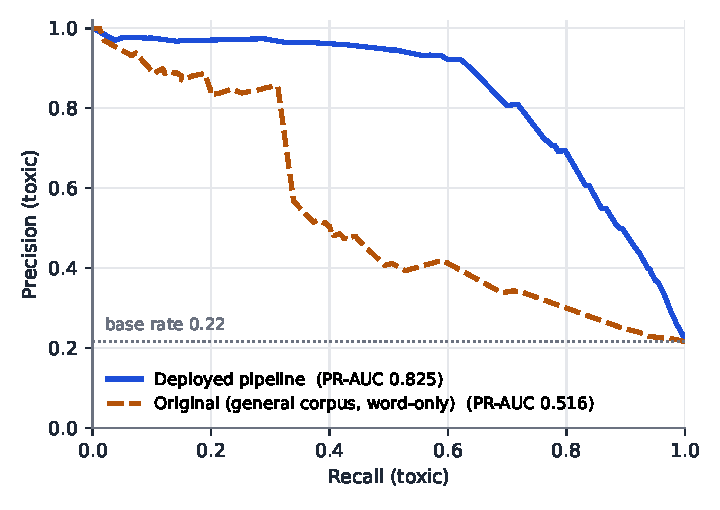
\includegraphics[width=0.9\linewidth]{pr_chat.pdf}
\caption{Precision--recall on held-out real gaming chat (CONDA validation split).
The deployed pipeline dominates the original general-corpus recipe across the curve.}
\label{fig:pr}
\end{figure}

\begin{figure*}[t]
\centering
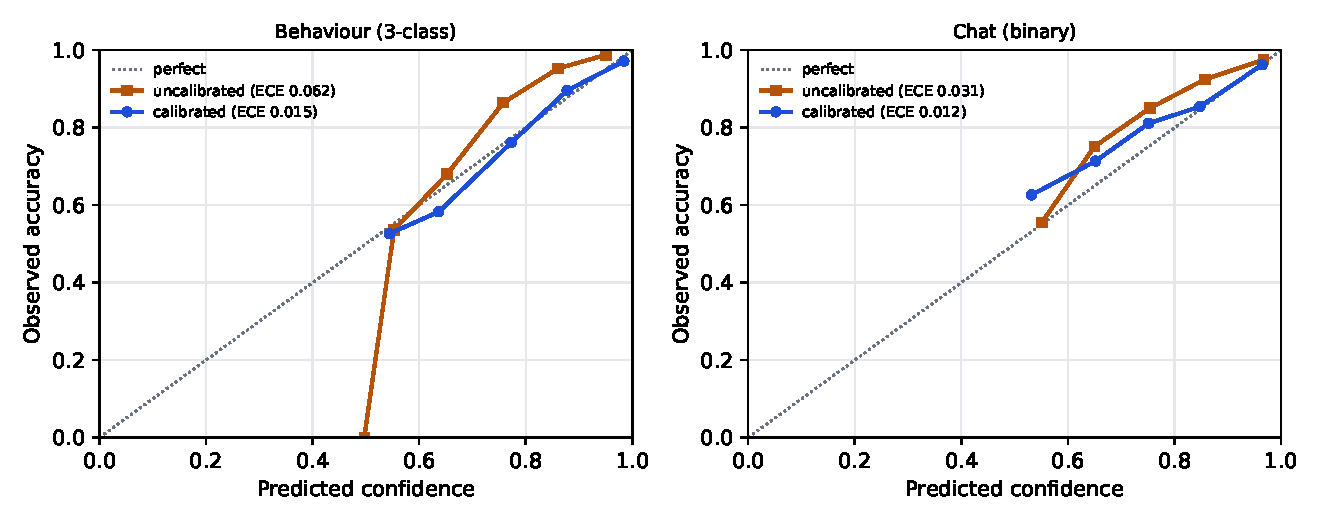
\includegraphics[width=0.85\textwidth]{reliability.pdf}
\caption{Reliability diagrams (top-label, 10 bins) for both calibrated channels.
Calibration cuts behaviour ECE $0.062\!\rightarrow\!0.015$ and chat $0.031\!\rightarrow\!0.012$.}
\label{fig:rel}
\end{figure*}

\subsection{External construct validation}\label{sec:survey}
Every behaviour-model number above is measured against synthetic labels, so the central
claim --- that \emph{how} a person plays carries screening signal that \emph{how long}
does not --- had never met a real instrument. We ran an anonymous, adults-only web
survey pairing the nine IGDS9-SF items~\cite{igds9sf} with seven multiple-choice
gaming-pattern questions that map onto the ten objective features by documented band
midpoints. Each respondent was scored through the \emph{deployed serving path} (shared
derivation, fitted scaler, calibrated forest, identical risk formula). $112$ raw
responses yielded $87$ usable (17 failed eligibility, 8 an attention check); $86$ were
scoreable. IGDS totals averaged $17.6$ (SD $6.1$; range $9$--$37$); one respondent was
in the disordered range. The model was fitted before the survey existed and nothing was
tuned on it.

\begin{table}[t]
\centering\footnotesize
\caption{Construct validity against IGDS9-SF ($n{=}86$; Spearman, bootstrap 95\% CIs).}
\label{tab:survey}
\begin{tabular}{@{}lcc@{}}
\toprule
Predictor & $\rho$ & 95\% CI \\
\midrule
\textbf{Served risk score} & $\mathbf{0.352}$ & $[0.158, 0.521]$ \\
Self-reported hours/week (baseline) & $0.155$ & $[-0.057, 0.376]$ \\
\textbf{Paired difference} (model $-$ hours) & $\mathbf{+0.195}$ & $[+0.026, +0.372]$ \\
Partial (hours removed) & $0.349$ & $[0.149, 0.521]$ \\
\midrule
Pattern-feature composite & $0.358$ & $[0.160, 0.529]$ \\
Volume-feature composite & $0.202$ & $[-0.011, 0.395]$ \\
Toxic-chat involvement (chat premise) & $0.315$ & $[0.114, 0.498]$ \\
Excluding 8 straight-liners ($n{=}78$) & $0.290$ & $[0.080, 0.475]$ \\
\bottomrule
\end{tabular}
\end{table}

\begin{figure}[!htb]
\centering
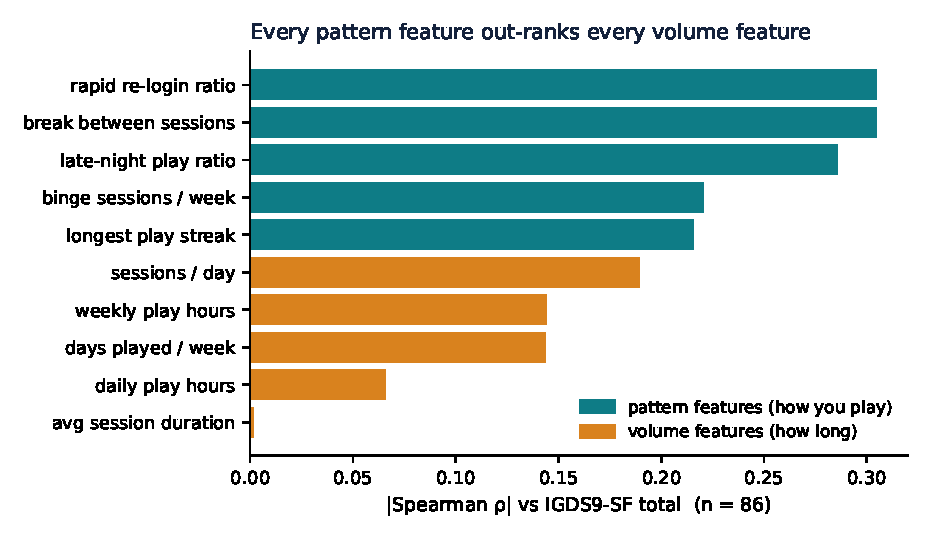
\includegraphics[width=\linewidth]{survey_features.pdf}
\caption{Per-feature $|\rho|$ against IGDS9-SF total. Every pattern feature out-ranks
every volume feature, with no interleaving.}
\label{fig:feat}
\end{figure}

\textbf{Results} (Table~\ref{tab:survey}, Fig.~\ref{fig:feat}). The served score
tracks the instrument at $\rho{=}0.352$, CI excluding zero. The screen-time baseline
every commercial tool ships reaches $0.155$ with a CI spanning zero; a paired bootstrap
puts the model ahead by $\Delta\rho{=}{+}0.195$ (CI excluding zero; model ahead in
$98.6\%$ of resamples), and partialling hours out barely moves it ($0.349$) --- the
score is not screen time in another unit. All five pattern features out-rank all five
volume features; the composites diverge ($0.358$ vs $0.202$, the latter's CI including
zero). Self-reported toxic-chat involvement tracks severity at $0.315$, replicating in
this population the $r{=}{+}0.156$ premise borrowed from~\cite{igdslatam2024}.
\textbf{Two results against the system.} The genre multiplier is unsupported
(Kruskal--Wallis across seven genres, $H{=}5.42$, $p{=}0.491$; power $36\%$, needing
$n\!\approx\!258$), so it is retained-and-flagged rather than defended --- removing it
flips $34\%$ of served bands. Four of five parent-facing proxies fail to track the IGDS
item they are named after (only ``craving'' holds, $\rho{=}0.325$); we renamed the
served labels to behaviour-descriptive wording. \textbf{Not established:} sensitivity /
specificity at the $\geq$$36$ cut-off (one positive; the analysis refuses caseness
metrics below ten by a guard written before the data arrived --- $\approx$$157$
usable responses are needed at the $6.4\%$ base rate); transfer to adolescents; any
longitudinal claim. A grid-searched threshold refit ($T_1{=}0.51,T_2{=}0.95$,
$\kappa{=}0.197$) was measured and \emph{declined}: $T_2$ is pinned by the sample's
missing severity tail, not a clinical boundary.

\textbf{What this validates, precisely --- and common-method variance.} The study
validates the served risk \emph{formula} applied to self-reported pattern answers
mapped to band midpoints; it does not yet validate the passive-sensing pipeline
end-to-end, whose inputs are measured telemetry rather than recalled bands. Because
both the predictor questions and the IGDS9-SF items are self-report from the same
respondent in one sitting, part of the association may be common-method
variance~\cite{podsakoff2003}. Three observations bound, without eliminating, that
concern: the incremental effect over self-reported hours ($\Delta\rho{=}{+}0.195$)
is a \emph{within-method} contrast, since hours are self-reported on the same form
and share any method inflation; the pattern-vs-volume separation is a
\emph{between-feature} contrast that shared method cannot manufacture; and the
predictor questions are behavioural frequencies, not attitudes, which typically
attenuates rather than inflates method effects. The clean test remains a
telemetry-linked cohort (\S V). On magnitude: $\rho{=}0.352$ ($\approx$$12\%$ shared
variance) is modest in absolute terms, with a wide interval at $n{=}86$; it sits
inside the $0.3$--$0.5$ range that criterion-validity coefficients for brief
behavioural screeners against full instruments typically
occupy~\cite{kroenke2003,cohen1988}, and is reported as evidence that the score
carries the intended construct, not as evidence of clinical accuracy.

\subsection{Accent-fairness audit of the spoken-chat path}
A transcription error that \emph{creates} a slur would concentrate false accusations on
whoever the acoustic model serves worst. We transcribed all $6{,}656$ clips of
Svarah~\cite{svarah2023} (9.6~h, 117 speakers, 65 districts) with the deployed
recogniser and pushed every hypothesis through the served scorer at $0.95$. Result:
\textbf{zero} false toxicity alerts in every accent group (rule-of-three bound
$\leq0.045\%$ overall) despite a $38.6\%$ overall WER --- the chain degrades toward
silence, not accusation. But coverage is not accent-uniform: WER is $34.6\%$ for
Dravidian-L1 speakers, $38.1\%$ Indo-Aryan, and $60.8\%$ Tibeto-Burman
(Tamil $30.9\%$ $\rightarrow$ Bodo $60.8\%$; gender balanced at $38.4/38.7\%$). The
equity issue is a recall gap on Northeast-Indian accents, named as the highest-leverage
STT improvement.

\subsection{System testing and on-device cost}
290 automated tests run in CI (180 backend on SQLite \emph{and} Postgres~16; 110
Android JVM; 7 research-integrity guards pinning the paper's numbers to the committed
JSONs). A concurrency smoke of 288 mixed requests over 24 threads produced zero errors
(p50 66~ms); the API was property-fuzzed, CVE-audited, and both signed APKs passed a
MobSF~\cite{mobsf} static audit. On a Galaxy M52 (two 15-min Roblox sessions, per-minute
sampling), the default monitoring path costs $\approx$$14\%$ of one core and
$288$/$301$~MB mean/peak PSS with no thermal throttling --- one-fifteenth of the game's
own $215\%$ --- whereas the dual Hindi+English STT toggle costs $51$--$72\%$ and
$399$/$419$~MB, \emph{failing} our acceptance gate on two of three criteria; it
therefore ships default-off. A consented single-family pilot ran 23 days in production
(60 alerts across all eight types; the fail-closed consent rotation exercised live).

% =====================================================================
\section{Ethics and Limitations}
\textbf{Ethics statement.} The consented family pilot was an engineering pilot within
the authors' own extended family and did not seek institutional review; no clinical
conclusions are drawn from it. The IGDS9-SF survey was anonymous, adults ($18+$)
only, collected no names, e-mail addresses or identifiers, displayed a consent
statement before the first item, and was voluntary; the supervising faculty member
was notified in writing before distribution. That is documented faculty
notification, \emph{not} an ethics-committee or IRB determination, and we do not
describe it as one; any cohort involving minors is gated on institutional review,
guardian consent and age-appropriate assent. Row-level responses are not released
(consent covered research use, not redistribution); aggregate outputs are.

The system is screening, not diagnosis, and every surface says so. It is scoped to
minors by design: a guardian with duty of care is what makes screening the unwilling
both possible and proportionate; an adult version is either a self-help journal or
spyware. Consent fails closed; export and deletion share one scope; raw audio is never
retained. We name three tensions rather than hide them. \emph{Sensing blind spots}:
detection is foreground-package-based, so games inside a browser or a host app's
webview are invisible; closing that gap requires screen capture or URL surveillance,
which we refuse --- a disclosed boundary beats a privacy regression. \emph{The
crisis asymmetry}: profanity alerts a parent, but a self-harm disclosure to the in-app
companion does not; this is a deliberate refusal to hard-code a contested clinical
judgement, and the tiered ``wellbeing check'' design is documented as a proposal
pending clinical review. \emph{Evidence limits}: behavioural training labels are
synthetic, so the $0.916$ is a separability figure that the survey does not upgrade;
what the survey upgrades is the claim that the score \emph{means} something. Caseness
accuracy is uncomputed, the cohort is adults, the design cross-sectional, and the
voice model trained on acted adult speech. A per-child cohort linking guardian-reported
IGDS9-SF to measured telemetry is the outstanding, ethics-gated instrument.

% =====================================================================
\section{Conclusion}
We built and deployed a multimodal gaming-addiction screening platform that moves
beyond screen time to measured behaviour, code-mixed chat toxicity and voice, fused
into a calibrated, explainable signal a parent can act on. Every model choice is
backed by held-out evidence and ablations; the pipeline's output is then anchored
outside its own training distribution against a clinical instrument, where the design
premise --- pattern over volume --- survives contact with real labels while two of its
components do not, and we publish both. The contribution is not a solved clinical
instrument; it is a fully built, transparently measured screening pipeline in which every
claim traces to a runnable script. The gap that remains is data, not architecture.

% =====================================================================
\begin{thebibliography}{00}
\bibitem{icd11} World Health Organization, \emph{International Classification of Diseases
11th Revision (ICD-11)} --- Gaming disorder (6C51), 2019.
\bibitem{igds9sf} H. M. Pontes and M. D. Griffiths, ``Measuring DSM-5 Internet Gaming
Disorder: Development and validation of a short psychometric scale,'' \emph{Computers in
Human Behavior}, vol.\ 45, pp.\ 137--143, 2015.
\bibitem{igdslatam2024} J. A. Bland\'on-Casta\~no, D. X. Puerta-Cort\'es, A. Carmona,
J. Ivern, L. W. Vilca, X. Carbonell, and T. Caycho-Rodr\'iguez, ``Cross-cultural invariance of
the Internet Gaming Disorder Scale--Short-Form (IGDS9-SF) in seven Latin American countries,''
\emph{Int.\ J.\ Mental Health and Addiction}, vol.~23, no.~6, pp.~4690--4715, 2024;
open dataset: \texttt{doi:10.17605/OSF.IO/GWCSN}.
\bibitem{shap2017} S. M. Lundberg and S.-I. Lee, ``A unified approach to interpreting
model predictions,'' in \emph{Advances in Neural Information Processing Systems
(NeurIPS)}, 2017.
\bibitem{conda2021} H. Weld \emph{et al.}, ``CONDA: a CONtextual Dual-Annotated dataset
for in-game toxicity understanding and detection,'' in \emph{Findings of ACL-IJCNLP},
2021.
\bibitem{davidson2017} T. Davidson, D. Warmsley, M. Macy, and I. Weber, ``Automated hate
speech detection and the problem of offensive language,'' in \emph{Proc.\ ICWSM}, 2017.
\bibitem{jigsaw2018} Jigsaw / Conversation AI, ``Toxic Comment Classification
Challenge'' (Wikipedia talk-page comments with crowd-sourced toxicity annotations),
Kaggle, 2018.
\bibitem{hasoc2019} T. Mandl, S. Modha, P. Majumder, D. Patel, M. Dave, C. Mandlia,
and A. Patel, ``Overview of the HASOC track at FIRE 2019: Hate speech and offensive
content identification in Indo-European languages,'' in \emph{Proc.\ FIRE}, 2019.
\bibitem{svarah2023} T. Javed, S. Joshi, V. Nagarajan, S. Sundaresan, J. Nawale,
M. Raman, K. Kumar, P. Kumar, and M. M. Khapra, ``Svarah: Evaluating English ASR
systems on Indian accents,'' in \emph{Proc.\ INTERSPEECH}, 2023.
\bibitem{detoxify2020} L. Hanu and Unitary team, ``Detoxify: toxic comment
classification models,'' open-source software,
\texttt{github.com/unitaryai/detoxify}, 2020.
\bibitem{vosk} Alpha Cephei, ``Vosk speech recognition toolkit,'' open-source
software, \texttt{alphacephei.com/vosk}.
\bibitem{bohra2018} A. Bohra, D. Vijay, V. Singh, S. S. Akhtar, and M. Shrivastava,
``A dataset of Hindi-English code-mixed social media text for hate speech
detection,'' in \emph{Proc.\ NAACL PEOPLES Workshop}, 2018.
\bibitem{studentlife2014} R. Wang, F. Chen, Z. Chen, T. Li, G. Harari, S. Tignor,
X. Zhou, D. Ben-Zeev, and A. T. Campbell, ``StudentLife: Assessing mental health,
academic performance and behavioral trends of college students using smartphones,''
in \emph{Proc.\ ACM UbiComp}, 2014.
\bibitem{wikihi} Wikimedia Foundation, ``Hindi Wikipedia,'' 20231101 snapshot
(CC-BY-SA), accessed via the \texttt{wikimedia/wikipedia} dataset, 2026.
\bibitem{ravdess2018} S. R. Livingstone and F. A. Russo, ``The Ryerson Audio-Visual
Database of Emotional Speech and Song (RAVDESS),'' \emph{PLoS ONE}, vol.\ 13, no.\ 5,
2018.
\bibitem{cremad2014} H. Cao, D. G. Cooper, M. K. Keutmann, R. C. Gur, A. Nenkova, and
R. Verma, ``CREMA-D: Crowd-sourced emotional multimodal actors dataset,'' \emph{IEEE
Trans.\ Affective Computing}, vol.~5, no.~4, 2014.
\bibitem{emodb2005} F. Burkhardt, A. Paeschke, M. Rolfes, W. F. Sendlmeier, and B. Weiss,
``A database of German emotional speech,'' in \emph{Proc.\ Interspeech}, 2005.
\bibitem{urdu2018} S. Latif, A. Qayyum, M. Usman, and J. Qadir, ``Cross lingual speech
emotion recognition: Urdu vs.\ Western languages,'' in \emph{Proc.\ Int.\ Conf.\ on
Frontiers of Information Technology (FIT)}, 2018.
\bibitem{mobsf} A. Abraham \emph{et al.}, ``Mobile Security Framework (MobSF),''
open-source software, \texttt{github.com/MobSF/Mobile-Security-Framework-MobSF}.
\bibitem{huang2024} Y. Huang, R. Wu, Y. Huang, Y. Xiang, and W. Zhou,
``Investigating mechanisms of Internet Gaming Disorder and developing intelligent
monitoring models using artificial intelligence technologies,'' \emph{BMC Public
Health}, 2024.
\bibitem{strojny2024} P. Strojny, K. Kapela, N. Lipp, and S. Sikstr\"om, ``Use of four
open-ended text responses to help identify people at risk of gaming disorder,'' \emph{JMIR
Serious Games}, vol.\ 12, e56663, 2024.
\bibitem{ergin2025} D. A. Ergin and C. A. Essau, ``Family factors and Internet Gaming
Disorder among adolescents: A systematic review,'' \emph{Int.\ J.\ Developmental
Science}, 2025.
\bibitem{podsakoff2003} P. M. Podsakoff, S. B. MacKenzie, J.-Y. Lee, and N. P. Podsakoff,
``Common method biases in behavioral research: A critical review of the literature and
recommended remedies,'' \emph{J. Applied Psychology}, vol.~88, no.~5, pp.~879--903, 2003.
\bibitem{kroenke2003} K. Kroenke, R. L. Spitzer, and J. B. W. Williams, ``The Patient Health
Questionnaire-2: Validity of a two-item depression screener,'' \emph{Medical Care},
vol.~41, no.~11, pp.~1284--1292, 2003.
\bibitem{cohen1988} J. Cohen, \emph{Statistical Power Analysis for the Behavioral Sciences},
2nd ed. Hillsdale, NJ: Lawrence Erlbaum, 1988.

\end{thebibliography}

\end{document}
